\subsection{Question 4}

\subsubsection*{Sketching out our functions} 
We're interested in the behaviour of the function 
\[ 
f(m) = \alpha_2 (T) m^2 + \alpha_4 m^4 + \alpha_6 m^6, \quad \alpha_4 < 0 
\] We first differentiate and see where roots exist. 
\[
f ' ( m ) = 2 m ( \alpha_2 + 2 \alpha_4 m^2 + 3 \alpha_6 m ^ 4 ) 
\] This implies that $ m = 0 $ is always a stationary point. 
We focus our attention to solving for roots of the quadratic factor. 
Without caring abotu signs for now, solving the equation as 
a quadratic in $ m^ 2 $ then square rooting gives 
\[
m = \pm \sqrt{  - \frac{\alpha_4 }{3 \alpha_6 } \pm  \frac{1}{ 3 \alpha_6 } \sqrt{ \alpha_4^2 - 3 \alpha_6 \alpha_2 }} 
\] Now, the number of real solutions depends on signs. 
This equation has no real solutions when $ \alpha_2 > \frac{ \alpha_4 }{ 3 \alpha_6 }$. 
Thus, $ m = 0 $ is our only stationary point. Our function is 

\begin{figure}[h]
\centering
\begin{tikzpicture}[scale=0.7]
\begin{axis}[ 
xlabel=$m$,
ylabel={$f(m)$}, 
axis x line=center,
axis y line=center,
ticks=none, 
no markers, 
clip=false 
] 
\addplot { x^6 }; 
\end{axis}
\end{tikzpicture} 
\end{figure} 

After this, we have only two real solutions 
in the case when  $ \alpha_2 < 0 $, is this implies that only 
$ \frac{ - \alpha_4 }{3 \alpha_6 } + \frac{1 }{ 3 \alpha_6 }\sqrt{ \alpha_4^2  - 3 \alpha_6 \alpha_2 } $ 
is positive in the square root. 
This means our only stationary points are at 0 and two other places. 
we know it's this shape since around zero, $m^2 $ term dominates and we should have a negative 
quadratic. 

\begin{figure}[h]
\centering
\begin{tikzpicture}[scale=0.8]
\begin{axis}[ 
samples=150, 
xlabel=$m$,
ylabel={$f(m)$}, 
axis x line=center,
axis y line=center,
ticks=none, 
no markers, 
restrict x to domain*=-2:2,
restrict y to domain*=-3:5,
xmin=-2,
xmax=2,
ymin=-3, 
ymax=5,
clip=false 
] 
\addplot {x^6 -   x^4  -  x^2 }; 
\end{axis}
\end{tikzpicture} 
\caption{This our metastable state disappears when $\alpha_2 ( T ) $ is below 0!}
\end{figure}

In our final case we have that for $ 0 < \alpha_2 < \frac{\alpha_4^2 }{3 \alpha_6 }$ 
we have five stationary points including zero. 
The only possible configurations for stationary points is that 
$ m_0  = 0, m_\pm  = \pm \sqrt{  - \frac{\alpha_4}{3\alpha_6 } + \frac{1}{3 \alpha_6 } \sqrt{ \alpha_4^2 - 3 \alpha_6 \alpha_2 } } $ 
must be minima, and the other points are maxima. 

Our condition for $ m_\pm$ to be \textbf{global} minima (not metastable states) 
is that we must have that $ f ( m_\pm) $ must be smaller than $ f (m_0 ) = 0 $. 
Algebra shows that 
\begin{align*}
m_\pm^2 & =  - \frac{\alpha_4}{\alpha_6 } + \frac{1}{ 3 \alpha_6 } \sqrt{ \alpha_4 ^ 2 - 3 \alpha_6 \alpha_2 } \\
m_\pm^ 4 & = \frac{1}{ 9 \alpha_6 ^ 2 } ( 2 \alpha_4 ^ 2 - 3 \alpha_6 \alpha_2  - 2 \alpha_4 \sqrt{ \alpha_4^2 - 3 \alpha_6 \alpha_2 } 
\end{align*}

So substituting this into $ f ( m ) $ gives 
 \begin{align*}
	 f ( m_\pm ) &= m_\pm^2 ( \alpha_2 + \alpha_4 \left(  - \frac{\alpha_4}{3 \alpha_6 } + \frac{1}{3\alpha_6 } \sqrt{ \alpha_4^  2 - 3 \alpha_6 \alpha_2}  \right) \\
		     & +  \frac{\alpha_6}{9 \alpha_6 ^ 2 } \left( 2 \alpha_4 ^ 2 - 3 \alpha_6 \alpha_2 - 2 \alpha_4 \sqrt{ \alpha_4 ^ 2  - 3 \alpha_6 \alpha_2 }  \right)) \\
		     &= m_\pm^2 ( \frac{ 2 \alpha_2 }{ 3 } - \frac{ \alpha_4^ 2 }{ 9 \alpha_6 } + \frac{\alpha_4 }{ 9 \alpha_6 } \sqrt{ \alpha_4  - 3 \alpha_6 \alpha_2} ) 
\end{align*}
Hence, we require that the term in the brackets is negative. 
If we multiply by $ 9 \alpha_6  > 0 $, our condition 
becomes that 
\begin{align*}
	6 \alpha_2 \alpha_6 - \alpha_4^ 2 + \alpha_4 \sqrt{ \alpha_4 ^ 2 - 3 \alpha_6 \alpha_2 }  & <  0  \\
	6 \alpha_2 \alpha_6- \alpha_4^ 2 <   - \alpha_4 \sqrt{ \alpha_4^  2 - 3 \alpha_2 \alpha_6 } 
\end{align*}
Squaring both sides, cancelling an $ \alpha_4 ^ 4 $ in the sum on each side,  and then cancelling 
$ \alpha_ 2 $ gives us the condition that 
 \[
  36 \alpha_2 \alpha_6 ^ 2 - 12 \alpha_4 ^ 2 \alpha_6 <  - 3 \alpha_4 ^ 2 \alpha 6 \implies \alpha_2 < \frac{ \alpha_4 ^ 2 }{4 \alpha_6 }
\] So, we get that our magnetisation jumps by $ m_\pm $ only when 
these points become a global minimum, at  $ \alpha_ 2  = \frac{\alpha_4 ^ 2 }{ 4 \alpha_6 }$ 

\begin{figure}[h]
	\centering
	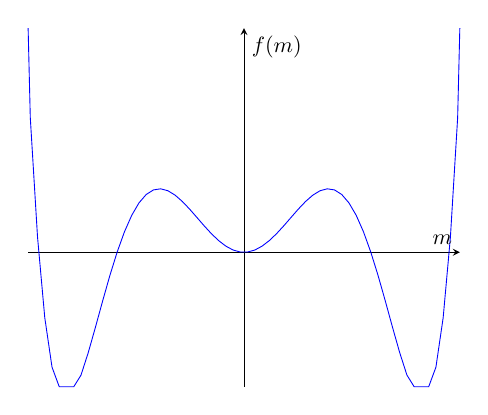
\begin{tikzpicture}[scale=0.8]
  \begin{axis}[ 
    samples=150, 
    xlabel=$m$,
    ylabel={$f(m)$}, 
    axis x line=center,
    axis y line=center,
    ticks=none, 
    no markers, 
    restrict x to domain*=-2:2,
    restrict y to domain*=-3:5,
    xmin=-2,
    xmax=2,
    ymin=-3, 
    ymax=5,
    clip=false 
  ] 
    \addplot {x^6 - 5 *  x^4 + 5 * x^2 }; 
  \end{axis}
\end{tikzpicture}
\quad 
	\begin{tikzpicture}[scale=0.8]
  \begin{axis}[ 
    samples=150, 
    xlabel=$m$,
    ylabel={$f(m)$}, 
    axis x line=center,
    axis y line=center,
    ticks=none, 
    no markers, 
    restrict x to domain*=-1.0:1.0,
    restrict y to domain*=-0.1:1.5,
    xmin=-1,
    xmax=1,
    ymin=-0.1, 
    ymax=1.5,
    clip=false 
  ] 
    \addplot {x^6 -  x^4 +0.3*  x^2 }; 
  \end{axis}
\end{tikzpicture}


 \caption{Left: when $ \frac{ \alpha_4^2}{ 4 \alpha_6} > \alpha_2 > 0$; we have a metastable state at $m = 0$. 
 On the right is what happens otherwise.}
\end{figure} 

Because of this jump, we have a phase transition. 

\subsubsection*{Showing a first order phase transition} 
For ease of notation let's denote the global minimum of $ f $
as  $ m_0 $ in either case. 
When $ \alpha_2 > \alpha_{ c } = \frac{ \alpha_4^ 2 }{4 \alpha_6 }$, we have $ f ( m _0 ) = 0$. 
Let's write our the energy in terms of $  m_0$ and differentiate with 
respect to the parameter $\alpha_2 $, denoted with an apostrophe. 
We have 
\begin{align*}
	f( m_0 ) &=  \alpha_2( T ) m_0^ 2 + \alpha_4 m_0 ^ 4 + \alpha_6 + m_0 ^ 6  \\
	f' ( m_ 0 ) & = 2 \alpha_2 m_0 m_0' + m_0^ 2 + 4\alpha_4 m_0 ^ 3 m_0' + 6 \alpha_6 m_0^ 5 m_0' \\
		    &=  m_0 ^ 2 + 2 m_0 m_0' (  \alpha_2 + 2 \alpha_4 m_0^ 2 + 3 \alpha_6 m_0 ^ 4 )  \\
		    &=  m_0 ^ 2  \\
\end{align*}
We took the last term to zero since $ m_0 $ solved this equation earlier. 
Now, if we take the limit as $ \alpha_2 \to \frac{ \alpha_4 ^ 2 }{4  \alpha_6 }$, 
it's easy to verify that 
\[
	m_0 =  - \frac{\alpha_4 }{3 \alpha_6 }+ \frac{1}{3 \alpha_6 }\sqrt{ \alpha_4^ 2 - 3 \alpha_2 \alpha_6 } \to  - \frac{1}{6 }\frac{\alpha_4 }{\alpha_6 }  
\] This is non zero. So, we have a discontinuity as we vary $ f( m_0 ) $ with respect to this parameter. 
\subsubsection*{Critical exponents} 
At $\alpha_4 = 0$, we have that 
\[ 
m \sim ( - \alpha_2)^{ \frac{ 1}{ 4} }  
\] 
The question is, how do we get a critical exponent from this with the condition that $\alpha(T_c)$  = 0? Critical exponents occur when $T \rightarrow T_c$, which means that $( T  - T_c)^2$ is small. We can Taylor expand $\alpha_2$ around the critical temperature as
\[ 
\alpha_ 2( T ) = \alpha_2(T_c) + ( T - T_c ) \alpha_2'(T_c) + \frac{ ( T - T_c)^2}{ 2} \alpha_2''(T_c) + \dots \sim ( T  - T_c) \text{ at leading order }
\] 
Substituting this in the expression above, we then must have that 
\[ 
m \sim ( T_c - T )^{ \frac{1}{4} } 
\] which implies that our critical exponent $\beta = \frac{1}{ 4} $ Now, for heat capacity, assuming that $\alpha_2 = K(T  - T_c ) $ to leading order, we have that our free energy can be written as 
\[ 
f(m) = \frac{  K^{ \frac{3}{2} } }{ ( 3 \alpha_6 )^ \frac{ 1}{ 2}}(  T_c - T )^{ \frac{3}{2}} + \frac{1 }{ 3 \alpha_6 } (T_c  - T )^3 
\] Now we can calculate our critical exponent for heat capacity! Heat capacity per unit volume is defined as 
\[ 
c = \frac{1}{N } \beta^2 \frac{ \partial }{ \partial \beta^2 } \log Z  = \left(  T^2 \frac{ \partial^2 }{ \partial T^2 } + 2T \frac{ \partial }{ \partial T } \right) \frac{ 1}{ T} f(m)
\] However, recall that since we're eventually taking a limit as $T \rightarrow T_c$, we only need to find the leading order contribution of $(T_c - T)^k$ from our expression above. This is akin to just differentiating the $( T_c - T ) terms $, and not caring about anything else. So, differentiating the first term twice in our expression for $f(m)$ gives a leading order contribution of $(T_c  - T)^{ - \frac{ 1}{2} } $, so $\alpha  = \frac{ 1}{2} $. 

To calculate $\delta$, observe that at the critical point with $\alpha_2 = 0$, our free energy is given by 
\[ 
f(m ) =  -B m + \alpha_6 m^6 
\] Solving for $f'(m) = 0 \implies \delta = 5$.  

To calculate our magnetisation constant, we define our new free energy as 
\[
g ( m )   = - Bm + \alpha_2 m^ 2 + \alpha_6 m ^ 6 
\] Consider the case when $\alpha_2 < 0 $.  We want to find our new minimum point such that this function is minimised. 
We work perturbatively. The minimum point $ m_0  \neq 0 $ for our free energy 
without magnetic field satisfies 
\[
f ( m )  = \alpha_2 m ^ 2  +\alpha_6 m ^ 6 \implies 0  = f' ( m_0 ) =  2m_0 ( \alpha_2 + 3 \alpha_6 m_0 ^ 4 ) 
\] We have that 
\[
g '( m ) = - B + 2m ( \alpha_2 + 3 \alpha_6 m ^ 4 ) 
\] We assume that our minimum point for small $B $ takes the form 
\[
m' = m_0 + \epsilon 
\] So, to first order in $ \epsilon$, we have 
\begin{align*}
 0 = g' ( m' ) &=  - B + ( m_0 + \epsilon) ( \alpha_2 + 3 \alpha_6 ( m_0 + \epsilon) ^ 4 ) \\
	       & = - B + 2 ( m_0 + \epsilon)( \alpha_2 + 3 \alpha_6 m_0^ 4 + 12 \alpha_6 \epsilon m_0^ 4) \\
	       &= - B + 2 ( m_0 + \epsilon) ( 0 + 12 \alpha_6 \epsilon m_0^3 ) \\
	       &= - B + 24 m_0^4 \epsilon \alpha_6 
	  \end{align*}
So, we have that 
\[
	\epsilon = \frac{B }{ 24 m_0^4 \alpha_6 } = \frac{B }{ 24 \alpha_2 \alpha_6} \sim \frac{B }{ 24 ( T_c - T )  \alpha_6} 
\] Hence, our equilibrium magnetisation is
\[
 m ' = m_0 +  \frac{B }{ 24 ( T_c - T )  \alpha_6} \implies  \xi =\frac{\partial m' }{\partial B } \sim \frac{1}{T_c - T }
\] This was for the case $ \alpha_2 < 0 $, where $ m_0 \neq 0 $. 
Otherwise, when $\alpha_2 > 0 $, $m \sim 0 $ and thus we can truncate $ g $
 \[
 g ( m) = - B m + \alpha_2 m^2 \implies m' = \frac{B}{2 \alpha_2 } \implies \xi  \sim \frac{1}{ T - T_c}
\] where $ m' $ is simply found by differentiating $g $ and setting to 0. 
Thus, on either side of the phase, 
\[
\xi \sim \frac{1}{ | T - T_c | } \implies \gamma = 1
\] 


\pagebreak 
